\chapter{Maximilian’s Avowal}

At the same moment M. de Villefort’s voice was heard calling from his
study, “What is the matter?”

Morrel looked at Noirtier who had recovered his self-command, and with
a glance indicated the closet where once before under somewhat similar
circumstances, he had taken refuge. He had only time to get his hat and
throw himself breathless into the closet when the procureur’s footstep
was heard in the passage.

Villefort sprang into the room, ran to Valentine, and took her in his
arms.

“A physician, a physician,—M. d’Avrigny!” cried Villefort; “or rather I
will go for him myself.”

He flew from the apartment, and Morrel at the same moment darted out at
the other door. He had been struck to the heart by a frightful
recollection—the conversation he had heard between the doctor and
Villefort the night of Madame de Saint-Méran’s death, recurred to him;
these symptoms, to a less alarming extent, were the same which had
preceded the death of Barrois. At the same time Monte Cristo’s voice
seemed to resound in his ear with the words he had heard only two hours
before, “Whatever you want, Morrel, come to me; I have great power.”

More rapidly than thought, he darted down the Rue Matignon, and thence
to the Avenue des Champs-Élysées.

Meanwhile M. de Villefort arrived in a hired cabriolet at M.
d’Avrigny’s door. He rang so violently that the porter was alarmed.
Villefort ran upstairs without saying a word. The porter knew him, and
let him pass, only calling to him:

“In his study, Monsieur Procureur—in his study!” Villefort pushed, or
rather forced, the door open.

“Ah,” said the doctor, “is it you?”

“Yes,” said Villefort, closing the door after him, “it is I, who am
come in my turn to ask you if we are quite alone. Doctor, my house is
accursed!”

“What?” said the latter with apparent coolness, but with deep emotion,
“have you another invalid?”

“Yes, doctor,” cried Villefort, clutching his hair, “yes!”

D’Avrigny’s look implied, “I told you it would be so.” Then he slowly
uttered these words, “Who is now dying in your house? What new victim
is going to accuse you of weakness before God?”

A mournful sob burst from Villefort’s heart; he approached the doctor,
and seizing his arm,—“Valentine,” said he, “it is Valentine’s turn!”

\begin{figure}[ht]
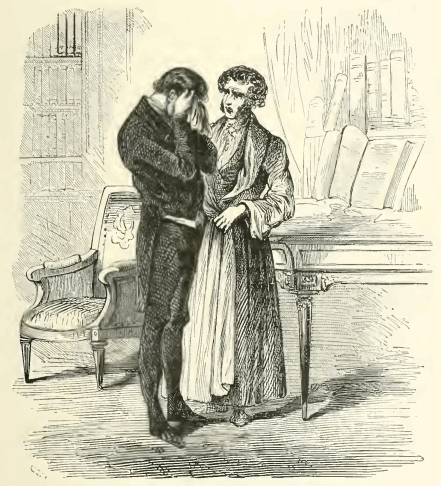
\includegraphics[width=\textwidth]{40284m.jpg}
\end{figure}

“Your daughter!” cried d’Avrigny with grief and surprise.

“You see you were deceived,” murmured the magistrate; “come and see
her, and on her bed of agony entreat her pardon for having suspected
her.”

“Each time you have applied to me,” said the doctor, “it has been too
late; still I will go. But let us make haste, sir; with the enemies you
have to do with there is no time to be lost.”

“Oh, this time, doctor, you shall not have to reproach me with
weakness. This time I will know the assassin, and will pursue him.”

“Let us try first to save the victim before we think of revenging her,”
said d’Avrigny. “Come.”

The same cabriolet which had brought Villefort took them back at full
speed, and at this moment Morrel rapped at Monte Cristo’s door.

The count was in his study and was reading with an angry look something
which Bertuccio had brought in haste. Hearing the name of Morrel, who
had left him only two hours before, the count raised his head, arose,
and sprang to meet him.

“What is the matter, Maximilian?” asked he; “you are pale, and the
perspiration rolls from your forehead.” Morrel fell into a chair.

“Yes,” said he, “I came quickly; I wanted to speak to you.”

“Are all your family well?” asked the count, with an affectionate
benevolence, whose sincerity no one could for a moment doubt.

“Thank you, count—thank you,” said the young man, evidently embarrassed
how to begin the conversation; “yes, everyone in my family is well.”

“So much the better; yet you have something to tell me?” replied the
count with increased anxiety.

“Yes,” said Morrel, “it is true; I have but now left a house where
death has just entered, to run to you.”

“Are you then come from M. de Morcerf’s?” asked Monte Cristo.

“No,” said Morrel; “is someone dead in his house?”

“The general has just blown his brains out,” replied Monte Cristo with
great coolness.

“Oh, what a dreadful event!” cried Maximilian.

“Not for the countess, or for Albert,” said Monte Cristo; “a dead
father or husband is better than a dishonored one,—blood washes out
shame.”

“Poor countess,” said Maximilian, “I pity her very much; she is so
noble a woman!”

“Pity Albert also, Maximilian; for believe me he is the worthy son of
the countess. But let us return to yourself. You have hastened to
me—can I have the happiness of being useful to you?”

\begin{figure}[ht]
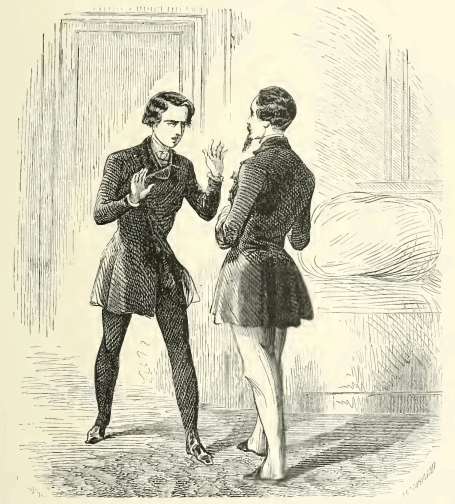
\includegraphics[width=\textwidth]{40286m.jpg}
\end{figure}

“Yes, I need your help: that is I thought like a madman that you could
lend me your assistance in a case where God alone can succor me.”

“Tell me what it is,” replied Monte Cristo.

“Oh,” said Morrel, “I know not, indeed, if I may reveal this secret to
mortal ears, but fatality impels me, necessity constrains me, count——”
Morrel hesitated.

“Do you think I love you?” said Monte Cristo, taking the young man’s
hand affectionately in his.

“Oh, you encourage me, and something tells me there,” placing his hand
on his heart, “that I ought to have no secret from you.”

“You are right, Morrel; God is speaking to your heart, and your heart
speaks to you. Tell me what it says.”

“Count, will you allow me to send Baptistin to inquire after someone
you know?”

“I am at your service, and still more my servants.”

“Oh, I cannot live if she is not better.”

“Shall I ring for Baptistin?”

“No, I will go and speak to him myself.” Morrel went out, called
Baptistin, and whispered a few words to him. The valet ran directly.

“Well, have you sent?” asked Monte Cristo, seeing Morrel return.

“Yes, and now I shall be more calm.”

“You know I am waiting,” said Monte Cristo, smiling.

“Yes, and I will tell you. One evening I was in a garden; a clump of
trees concealed me; no one suspected I was there. Two persons passed
near me—allow me to conceal their names for the present; they were
speaking in an undertone, and yet I was so interested in what they said
that I did not lose a single word.”

“This is a gloomy introduction, if I may judge from your pallor and
shuddering, Morrel.”

“Oh, yes, very gloomy, my friend. Someone had just died in the house to
which that garden belonged. One of the persons whose conversation I
overheard was the master of the house; the other, the physician. The
former was confiding to the latter his grief and fear, for it was the
second time within a month that death had suddenly and unexpectedly
entered that house which was apparently destined to destruction by some
exterminating angel, as an object of God’s anger.”

“Ah, indeed?” said Monte Cristo, looking earnestly at the young man,
and by an imperceptible movement turning his chair, so that he remained
in the shade while the light fell full on Maximilian’s face.

“Yes,” continued Morrel, “death had entered that house twice within one
month.”

“And what did the doctor answer?” asked Monte Cristo.

“He replied—he replied, that the death was not a natural one, and must
be attributed”—

“To what?”

“To poison.”

“Indeed!” said Monte Cristo with a slight cough which in moments of
extreme emotion helped him to disguise a blush, or his pallor, or the
intense interest with which he listened; “indeed, Maximilian, did you
hear that?”

“Yes, my dear count, I heard it; and the doctor added that if another
death occurred in a similar way he must appeal to justice.”

Monte Cristo listened, or appeared to do so, with the greatest
calmness.

“Well,” said Maximilian, “death came a third time, and neither the
master of the house nor the doctor said a word. Death is now, perhaps,
striking a fourth blow. Count, what am I bound to do, being in
possession of this secret?”

“My dear friend,” said Monte Cristo, “you appear to be relating an
adventure which we all know by heart. I know the house where you heard
it, or one very similar to it; a house with a garden, a master, a
physician, and where there have been three unexpected and sudden
deaths. Well, I have not intercepted your confidence, and yet I know
all that as well as you, and I have no conscientious scruples. No, it
does not concern me. You say an exterminating angel appears to have
devoted that house to God’s anger—well, who says your supposition is
not reality? Do not notice things which those whose interest it is to
see them pass over. If it is God’s justice, instead of his anger, which
is walking through that house, Maximilian, turn away your face and let
his justice accomplish its purpose.”

Morrel shuddered. There was something mournful, solemn, and terrible in
the count’s manner.

“Besides,” continued he, in so changed a tone that no one would have
supposed it was the same person speaking—“besides, who says that it
will begin again?”

“It has returned, count,” exclaimed Morrel; “that is why I hastened to
you.”

“Well, what do you wish me to do? Do you wish me, for instance, to give
information to the procureur?” Monte Cristo uttered the last words with
so much meaning that Morrel, starting up, cried out:

“You know of whom I speak, count, do you not?”

“Perfectly well, my good friend; and I will prove it to you by putting
the dots to the \textit{i}, or rather by naming the persons. You were walking
one evening in M. de Villefort’s garden; from what you relate, I
suppose it to have been the evening of Madame de Saint-Méran’s death.
You heard M. de Villefort talking to M. d’Avrigny about the death of M.
de Saint-Méran, and that no less surprising, of the countess. M.
d’Avrigny said he believed they both proceeded from poison; and you,
honest man, have ever since been asking your heart and sounding your
conscience to know if you ought to expose or conceal this secret. We
are no longer in the Middle Ages; there is no longer a Vehmgericht, or
Free Tribunals; what do you want to ask these people? ‘Conscience, what
hast thou to do with me?’ as Sterne said. My dear fellow, let them
sleep on, if they are asleep; let them grow pale in their drowsiness,
if they are disposed to do so, and pray do you remain in peace, who
have no remorse to disturb you.”

Deep grief was depicted on Morrel’s features; he seized Monte Cristo’s
hand. “But it is beginning again, I say!”

“Well,” said the Count, astonished at his perseverance, which he could
not understand, and looking still more earnestly at Maximilian, “let it
begin again,—it is like the house of the Atreidae;\footnote[19]{In the
old Greek legend the Atreidae, or children of Atreus, were doomed to
punishment because of the abominable crime of their father. The
\textit{Agamemnon} of Aeschylus is based on this legend.} God has condemned
them, and they must submit to their punishment. They will all
disappear, like the fabrics children build with cards, and which fall,
one by one, under the breath of their builder, even if there are two
hundred of them. Three months since it was M. de Saint-Méran; Madame de
Saint-Méran two months since; the other day it was Barrois; today, the
old Noirtier, or young Valentine.”

“You knew it?” cried Morrel, in such a paroxysm of terror that Monte
Cristo started,—he whom the falling heavens would have found unmoved;
“you knew it, and said nothing?”

“And what is it to me?” replied Monte Cristo, shrugging his shoulders;
“do I know those people? and must I lose the one to save the other?
Faith, no, for between the culprit and the victim I have no choice.”

“But I,” cried Morrel, groaning with sorrow, “I love her!”

“You love?—whom?” cried Monte Cristo, starting to his feet, and seizing
the two hands which Morrel was raising towards heaven.

“I love most fondly—I love madly—I love as a man who would give his
life-blood to spare her a tear—I love Valentine de Villefort, who is
being murdered at this moment! Do you understand me? I love her; and I
ask God and you how I can save her?”

Monte Cristo uttered a cry which those only can conceive who have heard
the roar of a wounded lion. “Unhappy man,” cried he, wringing his hands
in his turn; “you love Valentine,—that daughter of an accursed race!”

Never had Morrel witnessed such an expression—never had so terrible an
eye flashed before his face—never had the genius of terror he had so
often seen, either on the battle-field or in the murderous nights of
Algeria, shaken around him more dreadful fire. He drew back terrified.

As for Monte Cristo, after this ebullition he closed his eyes as if
dazzled by internal light. In a moment he restrained himself so
powerfully that the tempestuous heaving of his breast subsided, as
turbulent and foaming waves yield to the sun’s genial influence when
the cloud has passed. This silence, self-control, and struggle lasted
about twenty seconds, then the count raised his pallid face.

“See,” said he, “my dear friend, how God punishes the most thoughtless
and unfeeling men for their indifference, by presenting dreadful scenes
to their view. I, who was looking on, an eager and curious
spectator,—I, who was watching the working of this mournful tragedy,—I,
who like a wicked angel was laughing at the evil men committed
protected by secrecy (a secret is easily kept by the rich and
powerful), I am in my turn bitten by the serpent whose tortuous course
I was watching, and bitten to the heart!”

Morrel groaned.

“Come, come,” continued the count, “complaints are unavailing, be a
man, be strong, be full of hope, for I am here and will watch over
you.”

Morrel shook his head sorrowfully.

“I tell you to hope. Do you understand me?” cried Monte Cristo.
“Remember that I never uttered a falsehood and am never deceived. It is
twelve o’clock, Maximilian; thank heaven that you came at noon rather
than in the evening, or tomorrow morning. Listen, Morrel—it is noon; if
Valentine is not now dead, she will not die.”

“How so?” cried Morrel, “when I left her dying?”

Monte Cristo pressed his hands to his forehead. What was passing in
that brain, so loaded with dreadful secrets? What does the angel of
light or the angel of darkness say to that mind, at once implacable and
generous? God only knows.

Monte Cristo raised his head once more, and this time he was calm as a
child awaking from its sleep.

“Maximilian,” said he, “return home. I command you not to stir—attempt
nothing, not to let your countenance betray a thought, and I will send
you tidings. Go.”

“Oh, count, you overwhelm me with that coolness. Have you, then, power
against death? Are you superhuman? Are you an angel?” And the young
man, who had never shrunk from danger, shrank before Monte Cristo with
indescribable terror. But Monte Cristo looked at him with so melancholy
and sweet a smile, that Maximilian felt the tears filling his eyes.

“I can do much for you, my friend,” replied the count. “Go; I must be
alone.”

Morrel, subdued by the extraordinary ascendancy Monte Cristo exercised
over everything around him, did not endeavor to resist it. He pressed
the count’s hand and left. He stopped one moment at the door for
Baptistin, whom he saw in the Rue Matignon, and who was running.

Meanwhile, Villefort and d’Avrigny had made all possible haste,
Valentine had not revived from her fainting fit on their arrival, and
the doctor examined the invalid with all the care the circumstances
demanded, and with an interest which the knowledge of the secret
intensified twofold. Villefort, closely watching his countenance and
his lips, awaited the result of the examination. Noirtier, paler than
even the young girl, more eager than Villefort for the decision, was
watching also intently and affectionately.

At last d’Avrigny slowly uttered these words: “She is still alive!”

“Still?” cried Villefort; “oh, doctor, what a dreadful word is that.”

“Yes,” said the physician, “I repeat it; she is still alive, and I am
astonished at it.”

“But is she safe?” asked the father.

“Yes, since she lives.”

At that moment d’Avrigny’s glance met Noirtier’s eye. It glistened with
such extraordinary joy, so rich and full of thought, that the physician
was struck. He placed the young girl again on the chair,—her lips were
scarcely discernible, they were so pale and white, as well as her whole
face,—and remained motionless, looking at Noirtier, who appeared to
anticipate and commend all he did.

“Sir,” said d’Avrigny to Villefort, “call Mademoiselle Valentine’s
maid, if you please.”

Villefort went himself to find her; and d’Avrigny approached Noirtier.

“Have you something to tell me?” asked he. The old man winked his eyes
expressively, which we may remember was his only way of expressing his
approval.

“Privately?”

“Yes.”

“Well, I will remain with you.” At this moment Villefort returned,
followed by the lady’s maid; and after her came Madame de Villefort.

“What is the matter, then, with this dear child? she has just left me,
and she complained of being indisposed, but I did not think seriously
of it.”

The young woman with tears in her eyes and every mark of affection of a
true mother, approached Valentine and took her hand. D’Avrigny
continued to look at Noirtier; he saw the eyes of the old man dilate
and become round, his cheeks turn pale and tremble; the perspiration
stood in drops upon his forehead.

“Ah,” said he, involuntarily following Noirtier’s eyes, which were
fixed on Madame de Villefort, who repeated:

“This poor child would be better in bed. Come, Fanny, we will put her
to bed.”

M. d’Avrigny, who saw that would be a means of his remaining alone with
Noirtier, expressed his opinion that it was the best thing that could
be done; but he forbade that anything should be given to her except
what he ordered.

They carried Valentine away; she had revived, but could scarcely move
or speak, so shaken was her frame by the attack. She had, however, just
power to give one parting look to her grandfather, who in losing her
seemed to be resigning his very soul. D’Avrigny followed the invalid,
wrote a prescription, ordered Villefort to take a cabriolet, go in
person to a chemist’s to get the prescribed medicine, bring it himself,
and wait for him in his daughter’s room. Then, having renewed his
injunction not to give Valentine anything, he went down again to
Noirtier, shut the doors carefully, and after convincing himself that
no one was listening:

“Do you,” said he, “know anything of this young lady’s illness?”

“Yes,” said the old man.

“We have no time to lose; I will question, and do you answer me.”
Noirtier made a sign that he was ready to answer. “Did you anticipate
the accident which has happened to your granddaughter?”

“Yes.” D’Avrigny reflected a moment; then approaching Noirtier:

“Pardon what I am going to say,” added he, “but no indication should be
neglected in this terrible situation. Did you see poor Barrois die?”
Noirtier raised his eyes to heaven.

“Do you know of what he died!” asked d’Avrigny, placing his hand on
Noirtier’s shoulder.

“Yes,” replied the old man.

“Do you think he died a natural death?” A sort of smile was discernible
on the motionless lips of Noirtier.

“Then you have thought that Barrois was poisoned?”

“Yes.”

“Do you think the poison he fell a victim to was intended for him?”

“No.”

“Do you think the same hand which unintentionally struck Barrois has
now attacked Valentine?”

“Yes.”

“Then will she die too?” asked d’Avrigny, fixing his penetrating gaze
on Noirtier. He watched the effect of this question on the old man.

“No,” replied he with an air of triumph which would have puzzled the
most clever diviner.

“Then you hope?” said d’Avrigny, with surprise.

“Yes.”

“What do you hope?” The old man made him understand with his eyes that
he could not answer.

“Ah, yes, it is true,” murmured d’Avrigny. Then, turning to
Noirtier,—“Do you hope the assassin will be tried?”

“No.”

“Then you hope the poison will take no effect on Valentine?”

“Yes.”

“It is no news to you,” added d’Avrigny, “to tell you that an attempt
has been made to poison her?” The old man made a sign that he
entertained no doubt upon the subject. “Then how do you hope Valentine
will escape?”

Noirtier kept his eyes steadfastly fixed on the same spot. D’Avrigny
followed the direction and saw that they were fixed on a bottle
containing the mixture which he took every morning. “Ah, indeed?” said
d’Avrigny, struck with a sudden thought, “has it occurred to
you”—Noirtier did not let him finish.

“Yes,” said he.

“To prepare her system to resist poison?”

“Yes.”

“By accustoming her by degrees——”

“Yes, yes, yes,” said Noirtier, delighted to be understood.

“Of course. I had told you that there was brucine in the mixture I give
you.”

“Yes.”

“And by accustoming her to that poison, you have endeavored to
neutralize the effect of a similar poison?” Noirtier’s joy continued.
“And you have succeeded,” exclaimed d’Avrigny. “Without that precaution
Valentine would have died before assistance could have been procured.
The dose has been excessive, but she has only been shaken by it; and
this time, at any rate, Valentine will not die.”

A superhuman joy expanded the old man’s eyes, which were raised towards
heaven with an expression of infinite gratitude. At this moment
Villefort returned.

“Here, doctor,” said he, “is what you sent me for.”

“Was this prepared in your presence?”

“Yes,” replied the procureur.

“Have you not let it go out of your hands?”

“No.”

D’Avrigny took the bottle, poured some drops of the mixture it
contained in the hollow of his hand, and swallowed them.

“Well,” said he, “let us go to Valentine; I will give instructions to
everyone, and you, M. de Villefort, will yourself see that no one
deviates from them.”

\begin{figure}[ht]
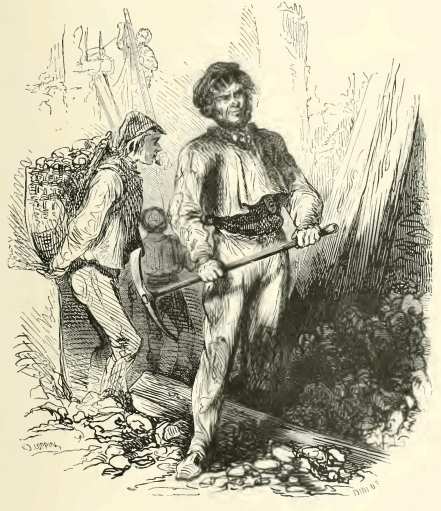
\includegraphics[width=\textwidth]{40294m.jpg}
\end{figure}

At the moment when d’Avrigny was returning to Valentine’s room,
accompanied by Villefort, an Italian priest, of serious demeanor and
calm and firm tone, hired for his use the house adjoining the hotel of
M. de Villefort. No one knew how the three former tenants of that house
left it. About two hours afterwards its foundation was reported to be
unsafe; but the report did not prevent the new occupant establishing
himself there with his modest furniture the same day at five o’clock.
The lease was drawn up for three, six, or nine years by the new tenant,
who, according to the rule of the proprietor, paid six months in
advance.

This new tenant, who, as we have said, was an Italian, was called Il
Signor Giacomo Busoni. Workmen were immediately called in, and that
same night the passengers at the end of the faubourg saw with surprise
that carpenters and masons were occupied in repairing the lower part of
the tottering house.
